\documentclass[12pt]{report}
\usepackage[utf8]{inputenc}
\usepackage{graphicx}
\usepackage{listings}
\usepackage{amsmath}
\usepackage{natbib}
\usepackage{float}
\usepackage{fancyhdr}

\pagestyle{fancy}
\fancyhf{}
\renewcommand{\footrulewidth}{0.4pt}% default is 0pt
\rhead{\rightmark}
\rfoot{Page \thepage}
\lfoot{Salvatore Cognetta, Artificial Intelligence and Robotics 2020/2021}

\begin{document}

\begin{titlepage}
    \centering
	
\includegraphics[width=0.5\textwidth]{cherubino.jpg}\par\vspace{1cm}
	\vspace{1cm}
	{\scshape\Large Reinforcement Learning implementation\par}
	\vspace{1.5cm}
	{\huge\bfseries DDPG + HER\par}
	\vspace{2cm}
	{\Large\itshape Salvatore Cognetta 1874383\par}
	\vfill    
    
	{\large \today\par}
\end{titlepage}

%\maketitle
\newpage
\tableofcontents
\newpage

\chapter{Algorithms}
\section{DDPG: Deep Deterministic Policy Gradient}
In real world scenarios, like pysical control tasks, there are continuous and high dimensional action spaces. Because it's not possible to apply Q-learning to continuous action spaces, caused by really slow optimization of the action $a_t$ at every timestep, DDPG was introduced.\\ 
DDPG is an algorithm which concurrently learns a Q-function and a policy. It uses off-policy data and the Bellman equation to learn the Q-function, and uses the Q-function to learn the policy.\\
This algorithm is based on DPG, which uses an actor-critic approach. In this approach there are two different functions: 
\begin{itemize}
	\item an actor function $\mu(s|\theta^\mu)$, which specifies the current policy mapping states to a specific action;
	\item a critic function $Q(s|a)$, which is learned using the Bellman equation.
\end{itemize}
Because the action space is continuous, and we assume the Q-function is differentiable with respect to action, to update the actor it's simply performed a gradient ascend:
\[
	\nabla_{\theta\mu}J \approx \frac{1}{N} \sum_i \nabla_a Q(s,a|\theta^Q)|_{s=s_i, a=\mu(s_i)} \nabla_{\theta^\mu}\mu(s|\theta^\mu)|_{s_i}
\]

\subsection{Target networks}
In DDPG are used neural network function approximators to learn state and action spaces online. Moreover, because Q learning with neural networks is very unstable in very environments, the paper propose a copy for actor-critic networks, called target networks $Q'(s,a|\theta^{Q'})$ and $\mu'(s|\theta^{\mu'})$, using soft target weights updates, instead of directly hard copying them. The weights of these target networks are updated accordingto the following rule: 
\[
	\theta' \leftarrow \tau \theta + (1-\tau)\theta'
\]

Therefore, the target values changes slowly, improving the stability of learning.

\subsection{Replay Buffer}
Using neural networks for reinforcement learning, althought introduces a new issue, in fact most optimization algorithms assume that the samples are independently and identically distributed. When the samples are generated from exploring sequentially, like in RL case, this assumption no longer holds. Moreover, to benefit from hardware optimizations, it's better to learn in mini-batches rather then online. To address this problems, the paper propose a replay buffer \textit{R}, a finite sized cache which stores the transitions, tuples containing $(s_t, a_t, r_t, s_{t+1})$. At each timestep, actor and critic are updated by sampling a minibatch from the buffer.

\subsection{Exploration and noise}
Because DDPG is an off-policy algorithm to make DDPG policies explore better, noise is added to their actions at training time. The authors of the original DDPG paper recommended time-correlated Ornestein-Uhlenbeck noise, but more recent results suggest that uncorrelated, mean-zero Gaussian noise works perfectly well. In this work there are implemented both, and one can choose by setting the variable $isOUNoise$ of the agent.\\
The resulting exploration policy is:
\[
	\mu'(s_t) = \mu(s_t|\theta_t^\mu) + N
\]

\subsection{Pseudocode}
\begin{figure}[H]
    \begin{center}
    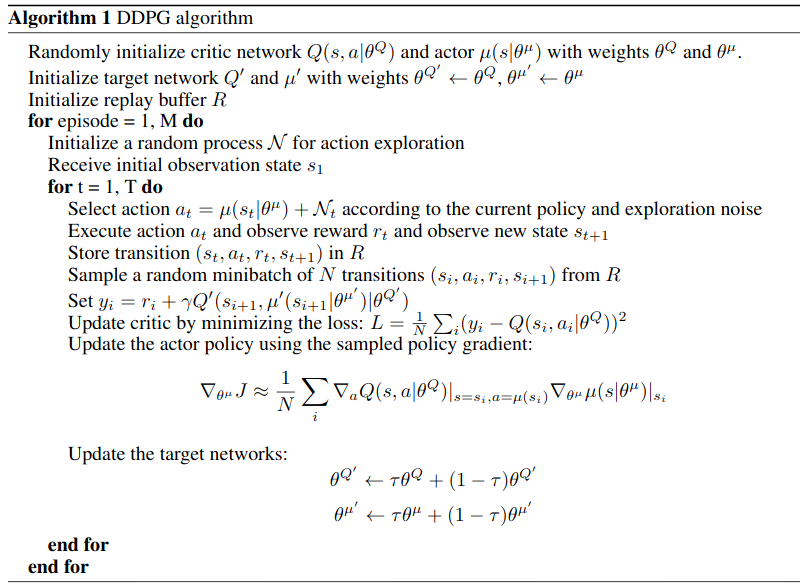
\includegraphics[scale=0.6]{ddpg_pseudocode.png}
    \end{center}
    \caption{DDPG pseudocode}
    \centering
\end{figure}


\section{HER: Hindsight Experience Replay}
The idea behind Hindsight Experience Replay (HER) is very simple: after experiencing some episode $s_0, s_1,..., s_T$ we store in the replay buffer every transition $s_t \rightarrow s_{t+1}$ not only with the original goal used for this episode but also with a subset of other goals. \\
There are different strategies for the additional goals:
\begin{itemize}
	\item \textbf{finite}: the only additional goals used for replay were the ones corresponding to the final state of the environment;
	\item future: replay with k random states which come from the same episode as the transition 	being replayed and were observed after it;
	\item random: replay with k random states encountered so far in the whole training procedure;
	\item episode: replay with k random states coming from the same episode as the transition			being replayed.
\end{itemize}
In this implementation the chosen goal is the final one of each episode.

\subsection{Pseudocode}
\begin{figure}[H]
    \begin{center}
    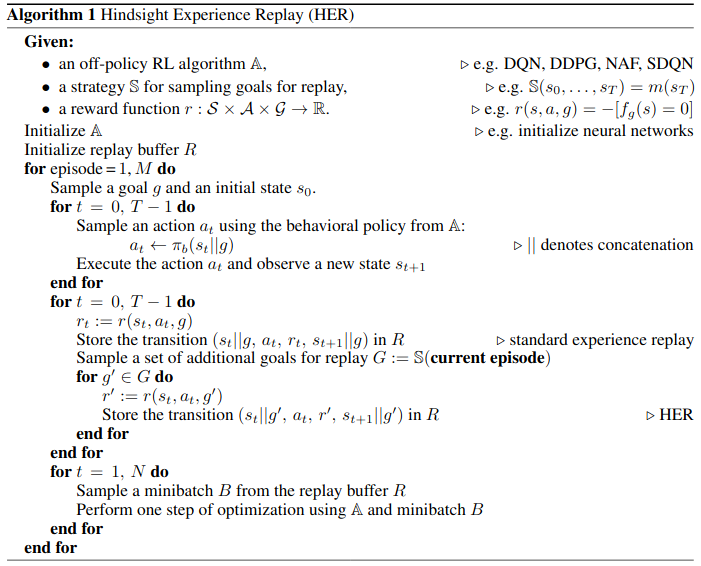
\includegraphics[scale=0.6]{her_pseudocode.png}
    \end{center}
    \caption{HER pseudocode}
    \centering
\end{figure}

\section{Implementation}
Different hyperparameters and the structure of the neural networks are taken from both papers.\\
For DDPG:
\begin{quotation}
	We used Adam (Kingma \& Ba, 2014) for learning the neural network parameters with a  learningrate of $10^{-4}$ and $10^{-3}$ for the actor and critic respectively. For $Q$ we included $L2$ weight decay of $10^{-2}$ and used a discount factor of $\gamma$ = 0.99. For the soft target updates we used $\tau$ = 0.001. The neural networks used the rectified non-linearity (Glorot et al., 2011) for all hidden layers. The final output layer of the actor was a tanh layer, to bound the actions. The low-dimensional networks had 2 hidden layers with 400 and 300 units respectively ($\approx$ 130,000 parameters). Actions were notincluded until the 2nd hidden layer of Q. When learning from pixels we used 3 convolutional layers(no pooling) with 32 filters at each layer.  This was followed by two fully connected layers with 200 units ($\approx$ 430,000 parameters). The final layer weights and biases of both the actor and criticwere initialized from a uniform distribution $[-3\times10^{-3},3\times10^{-3}]$ and $[3\times10^{-4},3\times10^{-4}]$ for the low dimensional and pixel cases respectively. This was to ensure the initial outputs for the policyand value estimates were near zero. The other layers were initialized from uniform distributions $[-\frac{1}{\sqrt{f}},\frac{1}{\sqrt{f}}]$ where f is the fan-in of the layer. The actions were not included until the fully-connected layers. We trained with minibatch sizes of 64 for the low dimensional problems and 16 on pixels. We used a replay buffer size of $10^6$.
	For the exploration noise process we used temporally correlated noise in order to explore well inphysical environments that have momentum.  We used an Ornstein-Uhlenbeck process (Uhlenbeck\& Ornstein, 1930) with $\theta$= 0.15 and $\sigma$= 0.2. 	
\end{quotation}
For HER:
\begin{quotation}
	We train for 200 epochs. Each epoch consists of 50 cycles where each cycle consists of running the policy for 16 episodes and then performing 40 optimization steps on mini batches of size 128 sampled uniformly from a replay buffer consisting of 106 transitions. We update the target networks after every cycle using the decay coefficient of 0.95. Apart from using the target network for computing Q-targets for the critic we also use it in testing episodes as it is more stable than the main network. The whole training procedure is distributed over 8 threads. For the Adam optimization algorithm we use the learning rate of 0.001.
\end{quotation}


\chapter{Environment} 
In this work the agent must be trained to perform the Fetch Pick And Place task, according to the DDPG + HER algorithm. This task consists of a robotic arm that has a gripper on the end-effector, this robo-arm must move in direction of a cube placed on a table, take it with the gripper hand and displace it to a specific goal.\\
This environment is taken from OpenAI Gym, using mujoco for the physic part.

\section{OpenAI Gym}
The OpenAI Gym framework makes available different kind of environments. After creating one of it, we can move according to a specified action (taken from our policy) with the step funcion. Each step returns an observation, a reward, a done boolean and finally an info array. \\
The $FetchPickAndPlace$, like all goal-based environments, uses a dictionary observation space.
It includes a desired goal, which the agent should attempt to achieve (desired\_goal), the goal that it has currently achieved instead (achieved\_goal), and the actual observation (observation), e.g. the state of the robot.

\chapter{Considerations}
Unfortunately the FetchPickAndPlace enviroment is not working as properly, probably because of some problem in her implementation. I've tried different experiments, but none of them seems improving the learning of this task. However the vanilla DDPG is working correctly, in fact it was tested on the Pendulum enviroment which brings to a very good result after only 200 epochs, as we can see in the image below.

\begin{figure}[H]
    \begin{center}
    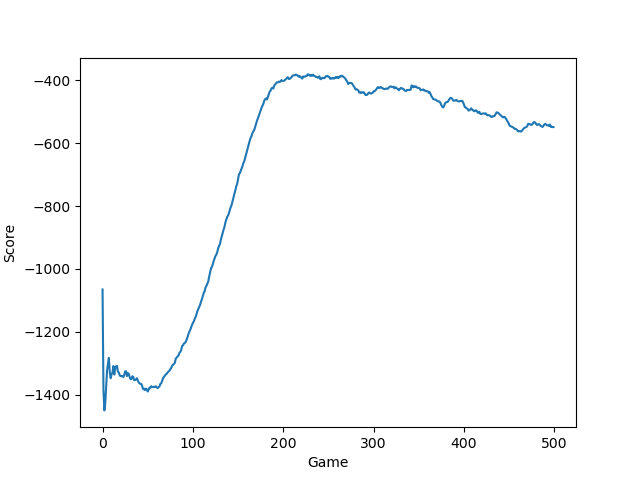
\includegraphics[scale=0.6]{Pendulum-v0.png}
    \end{center}
    \caption{Pendulum results}
    \centering
\end{figure}

\end{document}




